\documentclass[aspectratio=169,10pt]{beamer}

% ---- Encoding & fonts -----------------------------------------
\usepackage[utf8]{inputenc}
\usepackage[T1]{fontenc}
\usepackage{lmodern}

% ---- Theme ----------------------------------------------------
\usetheme{Madrid}
\usecolortheme{default}
\setbeamertemplate{navigation symbols}{}
\setbeamertemplate{footline}[frame number]

% ---- Packages -------------------------------------------------
\usepackage{booktabs}
\usepackage{listings}
\usepackage{xcolor}
\usepackage{tikz}
\usetikzlibrary{arrows.meta, positioning, shapes.geometric}
\usepackage{hyperref}
\usepackage{graphicx}
\graphicspath{{img/}}

% ---- Colors ---------------------------------------------------
\definecolor{codebg}{RGB}{245,245,248}
\definecolor{codekw}{RGB}{0,90,180}
\definecolor{codestr}{RGB}{160,50,50}
\definecolor{codered}{RGB}{180,30,30}
\definecolor{codegreen}{RGB}{30,120,60}
\definecolor{panelblue}{RGB}{40,90,160}
\definecolor{panelred}{RGB}{170,40,40}
\definecolor{panelgreen}{RGB}{40,130,70}
\definecolor{panelgray}{RGB}{90,90,90}

% ---- Listings (ASCII only) ------------------------------------
\lstdefinestyle{code}{
  basicstyle=\ttfamily\scriptsize,
  backgroundcolor=\color{codebg},
  keywordstyle=\color{codekw}\bfseries,
  stringstyle=\color{codestr},
  commentstyle=\color{codegreen}\itshape,
  numbers=none,
  frame=single,
  rulecolor=\color{gray!40},
  breaklines=true,
  columns=fullflexible,
  keepspaces=true,
  showstringspaces=false,
  extendedchars=false,
  upquote=true,
}
\lstset{style=code}

\title{Secure SQL AI Agent}
\subtitle{Plain-English database questions, safe by construction}
\author{Your Name}
\institute{Your Organisation}
\date{\today}

\begin{document}

% ===============================================================
\begin{frame}
  \titlepage
\end{frame}

% ===============================================================
\begin{frame}{The problem}
  \begin{block}{People want to ask the database in plain language}
    \emph{``Who are our top 3 customers by total spent?''}\\
    \emph{``Change the price of `Clean Code' to 39.''}\\
    \emph{``Which products have never been ordered?''}
  \end{block}

  \begin{alertblock}{Letting an LLM write SQL directly is dangerous}
    \begin{itemize}
      \item It can emit \texttt{DROP TABLE} or \texttt{DELETE} without a \texttt{WHERE}
      \item It invents tables and columns that do not exist
      \item A harmless-looking query can hide a write
            (\texttt{WITH d AS (DELETE ...) SELECT ...})
      \item Regex checks are easy to bypass --- SQL is a full language
    \end{itemize}
  \end{alertblock}
\end{frame}

% ===============================================================
\begin{frame}{The solution: three independent security layers}
  \begin{columns}[T]
    \begin{column}{0.32\textwidth}
      \begin{block}{\centering Layer 1}
        \centering\textbf{Static validation}\\[2pt]
        \footnotesize parse $\rightarrow$ policy $\rightarrow$ parameters\\
        $\rightarrow$ schema $\rightarrow$ EXPLAIN
      \end{block}
    \end{column}
    \begin{column}{0.32\textwidth}
      \begin{block}{\centering Layer 2}
        \centering\textbf{Human approval}\\[2pt]
        \footnotesize every write, with a one-time\\
        token bound to the exact SQL
      \end{block}
    \end{column}
    \begin{column}{0.32\textwidth}
      \begin{block}{\centering Layer 3}
        \centering\textbf{DB permissions}\\[2pt]
        \footnotesize read-only role vs writer role,\\
        enforced by PostgreSQL
      \end{block}
    \end{column}
  \end{columns}

  \vspace{8pt}
  \begin{alertblock}{Design principle}
    The LLM is \emph{untrusted input}. No single layer is trusted either:
    each one fails in a different way, so one failure is never enough.
  \end{alertblock}
\end{frame}

% ===============================================================
\begin{frame}{Architecture}
  \centering
  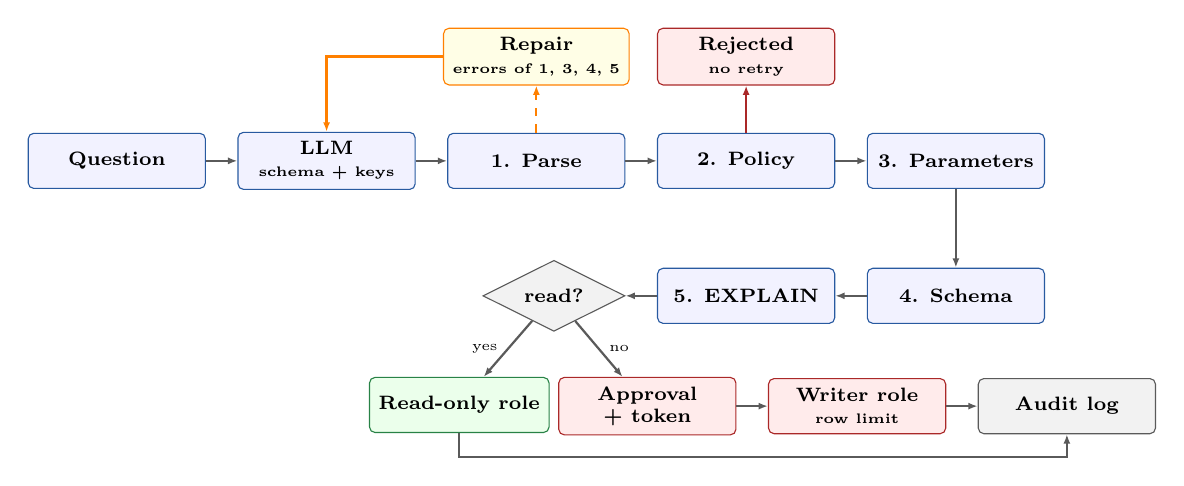
\begin{tikzpicture}[
    node distance=3mm and 4mm,
    box/.style={rectangle, rounded corners=2pt, draw=panelblue, fill=blue!5,
                minimum width=2.25cm, minimum height=7mm, font=\scriptsize\bfseries, align=center},
    decnode/.style={diamond, aspect=2, draw=panelgray, fill=gray!10,
                    minimum width=1.8cm, font=\scriptsize\bfseries, align=center},
    good/.style={box, fill=green!8, draw=panelgreen},
    bad/.style={box, fill=red!8, draw=panelred},
    arrow/.style={-{Latex[length=1.2mm]}, draw=panelgray, thick},
  ]
    \node[box] (user) {Question};
    \node[box, right=of user] (llm) {LLM\\\tiny schema + keys};
    \node[box, right=of llm] (parse) {1. Parse};
    \node[box, right=of parse] (pol) {2. Policy};
    \node[box, right=of pol] (par) {3. Parameters};

    \node[box, below=10mm of par] (sch) {4. Schema};
    \node[box, left=of sch] (exp) {5. EXPLAIN};
    \node[decnode, left=of exp] (dec) {read?};

    \node[good, below left=8mm and -4mm of dec] (ro) {Read-only role};
    \node[bad, below right=8mm and -4mm of dec] (appr) {Approval\\+ token};
    \node[bad, right=of appr] (wr) {Writer role\\\tiny row limit};
    \node[box, fill=gray!10, draw=panelgray, right=of wr] (audit) {Audit log};

    \node[bad, above=6mm of pol] (rej) {Rejected\\\tiny no retry};
    \node[box, fill=yellow!10, draw=orange, above=6mm of parse] (rep) {Repair\\\tiny errors of 1, 3, 4, 5};

    \draw[arrow] (user) -- (llm);
    \draw[arrow] (llm) -- (parse);
    \draw[arrow] (parse) -- (pol);
    \draw[arrow] (pol) -- (par);
    \draw[arrow] (par) -- (sch);
    \draw[arrow] (sch) -- (exp);
    \draw[arrow] (exp) -- (dec);
    \draw[arrow] (dec) -- node[left, font=\tiny]{yes} (ro);
    \draw[arrow] (dec) -- node[right, font=\tiny]{no} (appr);
    \draw[arrow] (appr) -- (wr);
    \draw[arrow] (wr) -- (audit);
    \draw[arrow, panelred] (pol) -- (rej);
    \draw[arrow, orange] (rep.west) -| (llm.north);
    \draw[arrow, orange, dashed] (parse.north) -- (rep.south);
    \draw[arrow] (ro.south) -- ++(0,-3mm) -| (audit.south);
  \end{tikzpicture}

  \vspace{6pt}
  {\footnotesize Everything after the LLM is deterministic Python. Mistakes go back
  to the model; forbidden requests are rejected immediately.}
\end{frame}

% ===============================================================
\begin{frame}{The validation pipeline}
  \centering
  \begin{tabular}{@{}llcl@{}}
    \toprule
    \textbf{Stage} & \textbf{Catches} & \textbf{Retry?} & \textbf{On failure} \\
    \midrule
    1. Parse      & syntax errors, 0 or 2+ statements                & yes & repair \\
    2. Policy     & DDL, dangerous functions, nested writes,         & \textbf{no} & \texttt{rejected} \\
                  & SELECT INTO, FOR UPDATE, EXPLAIN ANALYZE          &     & \\
    3. Parameters & missing values, \texttt{?} / \texttt{\$1}, \texttt{:x::int} & yes & repair \\
    4. Schema     & unknown tables / columns, ambiguous columns      & yes & repair \\
    5. EXPLAIN    & anything the PostgreSQL planner rejects          & yes & repair \\
    \midrule
    Write guard   & UPDATE/DELETE without a real \texttt{WHERE}      & no  & \texttt{rejected} \\
    \bottomrule
  \end{tabular}

  \vspace{4pt}
  {\footnotesize \emph{repair} = the failed SQL and the error are sent back to the LLM.}

  \vspace{6pt}
  \begin{block}{Why not retry everything?}
    \footnotesize
    A \emph{mistake} (wrong column name) is worth fixing. A \emph{forbidden request}
    (``drop the table'') would just produce another DROP --- retrying wastes
    time and money.
  \end{block}
\end{frame}

% ===============================================================
\begin{frame}[fragile]{Giving the model the right context}
  \begin{columns}[T]
    \begin{column}{0.55\textwidth}
      \begin{block}{\footnotesize Schema as the model sees it (\texttt{show\_schema})}
\begin{lstlisting}
TABLE public.customers (id INTEGER PK,
  email VARCHAR(255), full_name VARCHAR(150), ...)
TABLE public.orders (id INTEGER PK,
  customer_id INTEGER, status VARCHAR(20),
  total_amount NUMERIC(12, 2), ...)
  FK (customer_id) -> public.customers(id)
\end{lstlisting}
      \end{block}
      \footnotesize Primary and foreign keys tell the model how to JOIN ---
      in v0.1 they were collected but never sent.
    \end{column}
    \begin{column}{0.43\textwidth}
      \begin{block}{\footnotesize Rules in the prompt}
        \scriptsize
        \begin{itemize}
          \item one statement, JSON only
          \item only listed tables and columns
          \item every value as \texttt{:p\_name}
          \item \texttt{CAST(:p AS type)}, never \texttt{:p::type}
          \item explicit columns + \texttt{LIMIT}
          \item writes need a real \texttt{WHERE}
          \item impossible? return \texttt{"query": ""}
        \end{itemize}
      \end{block}
      \begin{block}{\footnotesize Model settings}
        \scriptsize temperature 0 \textperiodcentered{} JSON mode \textperiodcentered{}
        8k context for Ollama
      \end{block}
    \end{column}
  \end{columns}
\end{frame}

% ===============================================================
\begin{frame}[fragile]{Layer 1: classification on the syntax tree}
\begin{lstlisting}[language=Python]
def classify(self, tree):
    if isinstance(tree, exp.Command):          # EXPLAIN / SHOW
        return self._classify_command(tree)    # EXPLAIN ANALYZE / ANALYSE -> reject
    if dangerous_functions(tree):              # checked for EVERY statement type
        return unsupported("pg_sleep, pg_read_file, dblink, query_to_xml, ...")
    if isinstance(tree, (exp.Select, exp.Union, exp.Intersect, exp.Except)):
        return self._classify_read(tree)       # SELECT INTO, FOR UPDATE, hidden writes
    if isinstance(tree, (exp.Insert, exp.Update, exp.Delete, exp.Merge)):
        if contains_another_write(tree):       # WITH d AS (DELETE ...) INSERT ...
            return unsupported("nested write")
        return write()
    if isinstance(tree, DDL_NODES):
        return ddl() if ENABLE_DDL else unsupported("DDL disabled")
    return unsupported(type(tree).__name__)
\end{lstlisting}

  \begin{alertblock}{Allowlist, not blocklist}
    \footnotesize Only the statement shapes listed above can pass. Anything
    else --- \texttt{COPY}, \texttt{SET}, \texttt{DO \$\$...\$\$}, \texttt{VACUUM} --- is
    rejected because it is \emph{not} on the list.
  \end{alertblock}
\end{frame}

% ===============================================================
\begin{frame}[fragile]{Bounded writes}
  \begin{columns}[T]
    \begin{column}{0.52\textwidth}
\begin{lstlisting}[language=Python]
def is_potentially_unbounded_write(tree):
    if not isinstance(tree, (exp.Update, exp.Delete)):
        return False
    where = tree.args.get("where")   # OWN where only
    if where is None:
        return True
    return where.find(exp.Column) is None
\end{lstlisting}
    \end{column}
    \begin{column}{0.46\textwidth}
      \footnotesize
      \begin{tabular}{@{}lc@{}}
        \toprule
        \textbf{Statement} & \textbf{OK?} \\
        \midrule
        \texttt{... WHERE id = :p\_id}        & \textcolor{panelgreen}{yes} \\
        \texttt{DELETE FROM orders}           & \textcolor{panelred}{no} \\
        \texttt{... WHERE 1 = 1}              & \textcolor{panelred}{no} \\
        \texttt{SET x = (SELECT .. WHERE ..)} & \textcolor{panelred}{no} \\
        \bottomrule
      \end{tabular}
    \end{column}
  \end{columns}

  \vspace{8pt}
  \begin{block}{And after execution}
    \footnotesize
    The write runs in a transaction. If \texttt{rowcount > MAX\_WRITE\_ROWS} (default 100)
    it is \textbf{rolled back}. Statement and lock timeouts stop slow or blocked writes.
  \end{block}
\end{frame}

% ===============================================================
\begin{frame}[fragile]{Layer 2: one-time approval tokens}
\begin{lstlisting}[language=Python]
def create_token(request):
    token = secrets.token_urlsafe(32)
    self._pending[token] = ApprovalToken(
        sql_hash=sha256(request.sql),
        params_hash=sha256(json.dumps(request.parameters, sort_keys=True)))
    return token

def verify_and_consume(token, sql, params):
    stored = self._pending.pop(token, None)                 # one-time use
    if stored is None:                       raise ApprovalError("invalid or used")
    if stored.sql_hash != sha256(sql):       raise ApprovalError("different SQL")
    if stored.params_hash != sha256(params): raise ApprovalError("different parameters")
\end{lstlisting}

  \begin{alertblock}{Edits at the prompt are untrusted too}
    \footnotesize
    Edited SQL goes through \emph{every} check again --- validation, ``must still be a
    write'', the unbounded-write guard --- and gets a fresh approval prompt.
  \end{alertblock}
\end{frame}

% ===============================================================
\begin{frame}[fragile]{Layer 3: database-enforced permissions}
  \begin{columns}[T]
    \begin{column}{0.5\textwidth}
      \begin{block}{\footnotesize Read-only role}
\begin{lstlisting}[language=SQL]
GRANT SELECT ON ALL TABLES
  IN SCHEMA public TO sql_agent_readonly;
ALTER ROLE sql_agent_readonly
  SET default_transaction_read_only = on;
\end{lstlisting}
      \end{block}
    \end{column}
    \begin{column}{0.5\textwidth}
      \begin{block}{\footnotesize Writer role}
\begin{lstlisting}[language=SQL]
GRANT SELECT, INSERT, UPDATE, DELETE
  ON ALL TABLES IN SCHEMA public
  TO sql_agent_writer;
-- no CREATE, DROP, ALTER, TRUNCATE
\end{lstlisting}
      \end{block}
    \end{column}
  \end{columns}

  \begin{block}{\footnotesize The read path cannot write --- for three independent reasons}
    \footnotesize no write grants \textperiodcentered{} read-only role setting
    \textperiodcentered{} \texttt{SET TRANSACTION READ ONLY} on every read
  \end{block}

  \begin{alertblock}{\footnotesize The critical test, bypassing Python completely}
    \footnotesize
    \texttt{psql -U sql\_agent\_readonly -c "UPDATE products SET price = 0 WHERE id = 1"}\\
    \texttt{ERROR: cannot execute UPDATE in a read-only transaction}
  \end{alertblock}
\end{frame}

% ===============================================================
\begin{frame}[fragile]{One read request}
\begin{lstlisting}
You: top 3 customers by total spent

Generated SQL:
SELECT c.id, c.full_name, SUM(o.total_amount) AS total_spent
FROM customers c JOIN orders o ON o.customer_id = c.id
GROUP BY c.id, c.full_name ORDER BY total_spent DESC LIMIT 3;

Validation: [PASS] schema

+----+---------------+-------------+
| id | full_name     | total_spent |
+----+---------------+-------------+
| 1  | Alice Johnson | 3733.00     |
| 9  | Ivy Chen      | 1799.00     |
| 2  | Bob Smith     | 1149.00     |
+----+---------------+-------------+
Agent: Query executed successfully. 3 row(s) returned.
\end{lstlisting}
  {\footnotesize parsed $\rightarrow$ classified as read $\rightarrow$ columns resolved
  $\rightarrow$ \texttt{EXPLAIN} on the read-only role $\rightarrow$ executed $\rightarrow$ audited}
\end{frame}

% ===============================================================
\begin{frame}[fragile]{One write request}
\begin{lstlisting}
You: change the price of product 7 to 39

==========================================
          WRITE APPROVAL REQUIRED
==========================================
Operation: UPDATE
SQL:
UPDATE products SET price = :p_price WHERE id = :p_id;
Parameters:
  p_price = 39
  p_id = 7
Tables: products
1. Approve   2. Reject   3. Edit
==========================================
Approve? (yes/no/edit): yes

Agent: Write operation executed successfully. Affected rows: 1.
\end{lstlisting}
  \centering\footnotesize Before this prompt appeared, the UPDATE was already
  checked with \texttt{EXPLAIN} --- planned, never executed, rolled back.
\end{frame}

% ===============================================================
\begin{frame}[fragile]{Bounded self-repair}
\begin{lstlisting}
You: show each customer's age

[attempt 1] SELECT c.full_name, c.age FROM customers c
            -> schema: Column 'age' could not be resolved

[attempt 2] the model receives its SQL, its parameters and the problem
            -> {"query": "", "explanation": "There is no age or birth date column."}

Agent: I couldn't turn that into a database query.
\end{lstlisting}

  \begin{block}{Rules}
    \footnotesize
    \begin{itemize}
      \item the failed SQL is sent back, not only the error message
      \item every attempt goes through the full validation again
      \item at most \texttt{MAX\_SQL\_REPAIR\_ATTEMPTS} (default 2) retries
      \item ``I can't'' is an allowed answer --- better than an invented table
    \end{itemize}
  \end{block}
\end{frame}

% ===============================================================
\begin{frame}[fragile]{Ways to use it}
  \begin{columns}[T]
    \begin{column}{0.5\textwidth}
      \begin{block}{Interactive}
\begin{lstlisting}
uv run python -m app.main

You: how many orders are pending
You: sql top 5 products by revenue
You: show_schema
\end{lstlisting}
        \footnotesize \texttt{sql <question>} = generate and validate only,
        nothing runs.
      \end{block}
    \end{column}
    \begin{column}{0.5\textwidth}
      \begin{block}{One-shot / scripts}
\begin{lstlisting}
uv run python -m app.main \
  --sql-only "customers from Berlin"

uv run python -m app.main \
  --json "how many orders are pending"
\end{lstlisting}
        \footnotesize exit code 0 = success, 2 = rejected or failed
      \end{block}
    \end{column}
  \end{columns}

  \vspace{6pt}
  \begin{block}{Web interface}
    \footnotesize \texttt{uv run python -m app.web} $\rightarrow$ \texttt{http://127.0.0.1:8000}
  \end{block}
  \begin{block}{LLM providers}
    \footnotesize Ollama (local, free) \textperiodcentered{} OpenAI \textperiodcentered{}
    any OpenAI-compatible server (\texttt{OPENAI\_BASE\_URL}) \textperiodcentered{}
    mock (for tests)
  \end{block}
\end{frame}

% ===============================================================
\begin{frame}{Web interface}
  \begin{columns}[T]
    \begin{column}{0.5\textwidth}
      \centering
      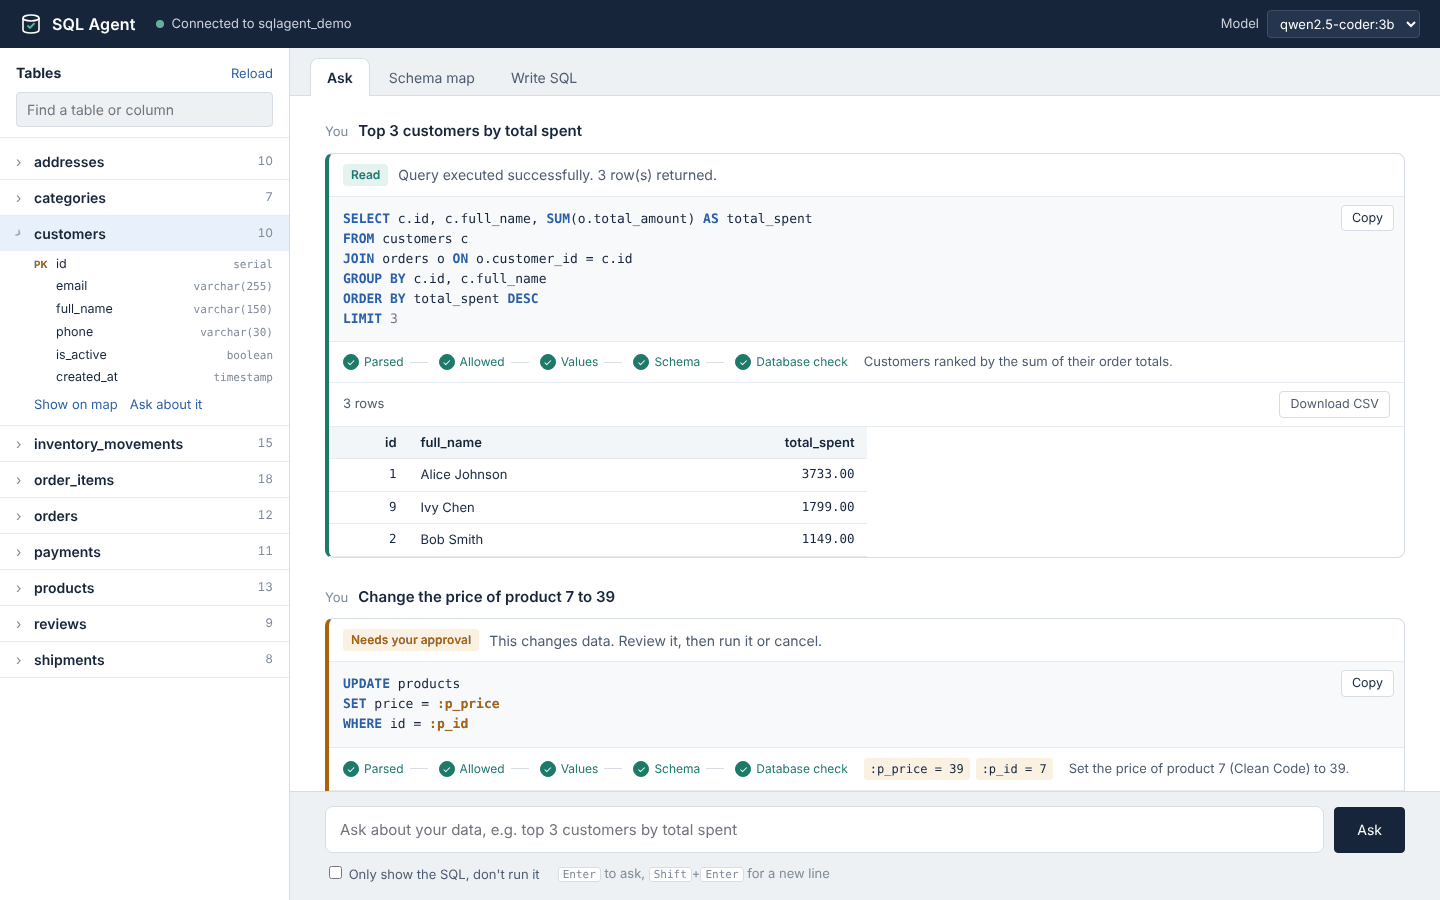
\includegraphics[width=\linewidth]{web-ask.png}\\[2pt]
      {\scriptsize Ask: SQL, the five checks, results; changes wait for approval}
    \end{column}
    \begin{column}{0.5\textwidth}
      \centering
      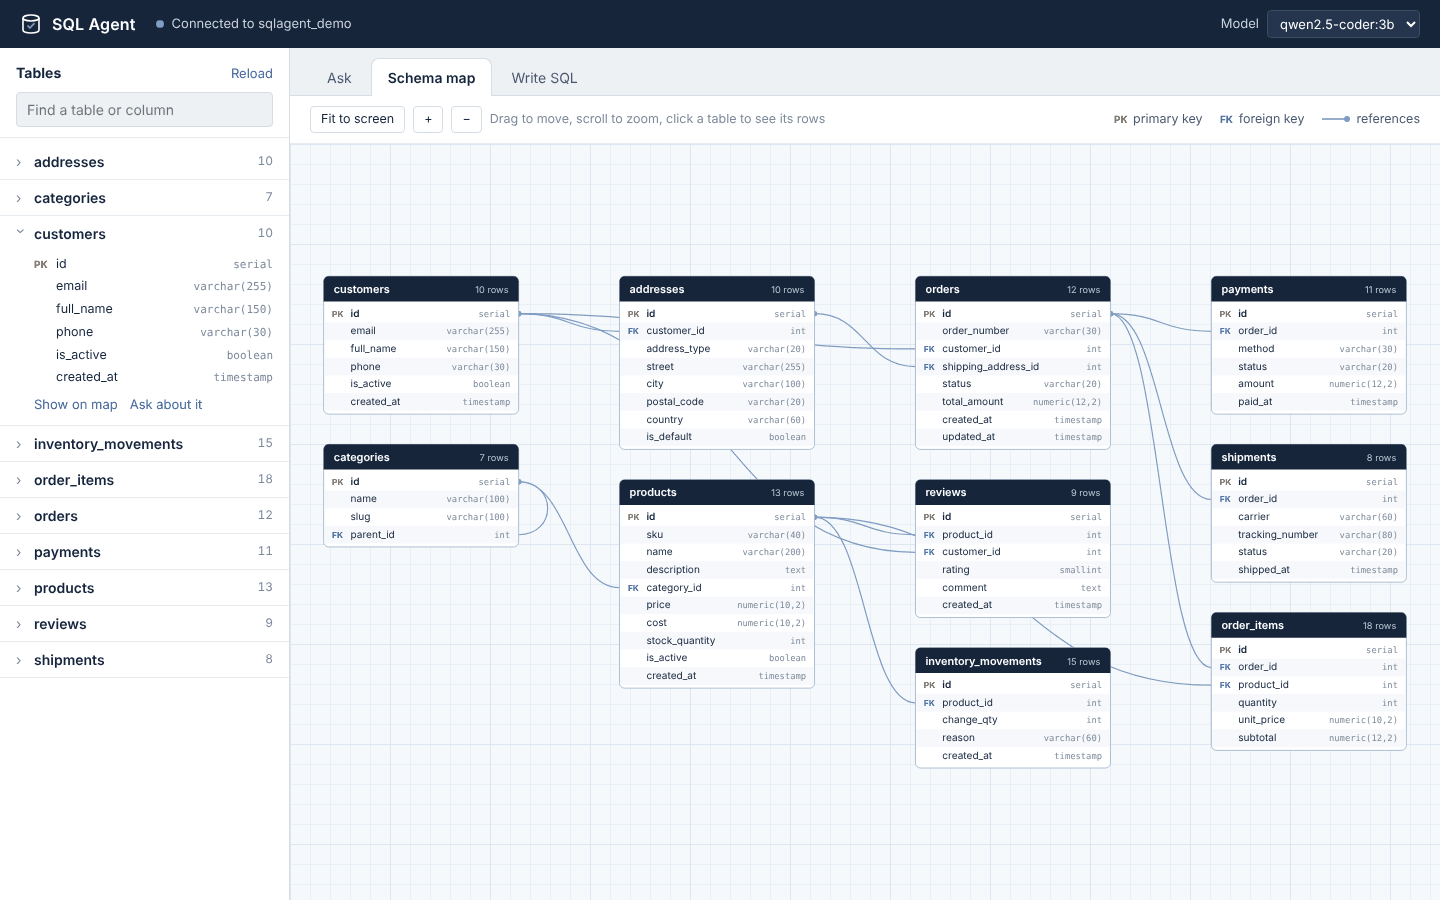
\includegraphics[width=\linewidth]{web-map.png}\\[2pt]
      {\scriptsize Schema map: tables, keys and relationships; click for rows}
    \end{column}
  \end{columns}

  \vspace{8pt}
  \begin{block}{}
    \footnotesize
    Table browser with row counts \textperiodcentered{} sortable results and CSV export
    \textperiodcentered{} hand-written SQL with the same checks \textperiodcentered{}
    switch Ollama models from the header \textperiodcentered{} no CDN, works offline
  \end{block}
\end{frame}

% ===============================================================
\begin{frame}{The browser chooses whether, never what}
  \centering
  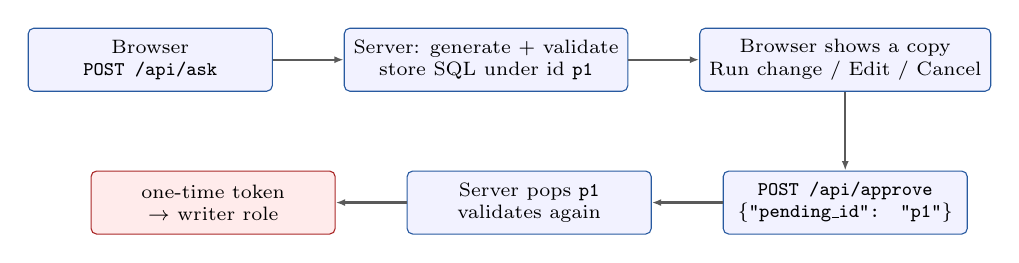
\begin{tikzpicture}[
    node distance=5mm and 9mm,
    box/.style={rectangle, rounded corners=2pt, draw=panelblue, fill=blue!5,
                minimum width=3.1cm, minimum height=8mm, font=\scriptsize, align=center},
    bad/.style={box, fill=red!8, draw=panelred},
    arrow/.style={-{Latex[length=1.2mm]}, draw=panelgray, thick},
  ]
    \node[box] (b1) {Browser\\\texttt{POST /api/ask}};
    \node[box, right=of b1] (s1) {Server: generate + validate\\store SQL under id \texttt{p1}};
    \node[box, right=of s1] (b2) {Browser shows a copy\\Run change / Edit / Cancel};
    \node[box, below=10mm of b2] (b3) {\texttt{POST /api/approve}\\\texttt{\{"pending\_id": "p1"\}}};
    \node[box, left=of b3] (s2) {Server pops \texttt{p1}\\validates again};
    \node[bad, left=of s2] (s3) {one-time token\\$\rightarrow$ writer role};
    \draw[arrow] (b1) -- (s1);
    \draw[arrow] (s1) -- (b2);
    \draw[arrow] (b2) -- (b3);
    \draw[arrow] (b3) -- (s2);
    \draw[arrow] (s2) -- (s3);
  \end{tikzpicture}

  \vspace{8pt}
  \begin{columns}[T]
    \begin{column}{0.48\textwidth}
      \begin{block}{\footnotesize Why}
        \footnotesize Approval carries only an id. Editing the HTTP request cannot
        change which SQL runs; each id works once and expires after 15 minutes.
      \end{block}
    \end{column}
    \begin{column}{0.48\textwidth}
      \begin{alertblock}{\footnotesize Limits}
        \footnotesize No login yet: the server listens on \texttt{127.0.0.1} only.
        Add authentication before sharing it.
      \end{alertblock}
    \end{column}
  \end{columns}
\end{frame}

% ===============================================================
\begin{frame}{Version 0.2: security fixes}
  \footnotesize
  \begin{tabular}{@{}p{5.6cm}p{6.2cm}@{}}
    \toprule
    \textbf{Problem in v0.1} & \textbf{Fix} \\
    \midrule
    Editing the SQL at the prompt to \texttt{DELETE FROM customers} executed it
      & all checks re-run after every edit \\
    \texttt{WHERE} inside a sub-query counted as a \texttt{WHERE}
      & only the statement's own \texttt{WHERE} counts; \texttt{WHERE 1=1} rejected \\
    Dangerous functions blocked only in SELECTs
      & blocked in every statement; list extended \\
    Write hidden in a CTE of another write
      & any nested write is rejected \\
    \texttt{EXPLAIN ANALYSE} (British spelling) passed
      & both spellings blocked \\
    Read-only role could be switched to read-write in a session
      & role-level \texttt{default\_transaction\_read\_only} \\
    \bottomrule
  \end{tabular}

  \vspace{6pt}
  \begin{alertblock}{}
    \footnotesize Every one of these passed the original tests. Each now has a regression
    test in \texttt{tests/test\_hardening.py}.
  \end{alertblock}
\end{frame}

% ===============================================================
\begin{frame}{Version 0.2: correctness and quality}
  \footnotesize
  \begin{columns}[T]
    \begin{column}{0.5\textwidth}
      \begin{block}{Bugs fixed}
        \begin{itemize}
          \item OpenAI provider failed on every request
          \item \texttt{INSERT} column names never checked
          \item \texttt{SELECT ID FROM Users} rejected (case)
          \item \texttt{UNION} queries rejected
          \item DDL could never succeed
          \item error messages showed \texttt{None}
          \item wrong port in \texttt{.env.example}
          \item crash on \texttt{refresh\_schema} when DB down
        \end{itemize}
      \end{block}
    \end{column}
    \begin{column}{0.5\textwidth}
      \begin{block}{New}
        \begin{itemize}
          \item prompt with PK/FK, shared by all providers
          \item parameter validation stage
          \item EXPLAIN for writes before approval
          \item repair loop sees its failed SQL
          \item policy failures not retried
          \item generate-only mode, one-shot CLI, table output
          \item streamed reads (server-side cursor)
          \item uv project setup
        \end{itemize}
      \end{block}
    \end{column}
  \end{columns}
\end{frame}

% ===============================================================
\begin{frame}{Live demo}
  \begin{columns}[T]
    \begin{column}{0.5\textwidth}
      \begin{block}{Reads (run immediately)}
        \footnotesize
        \begin{itemize}
          \item top 3 customers by total spent
          \item which products have never been ordered
          \item average rating per product
          \item pending orders from the last 30 days
        \end{itemize}
      \end{block}
      \begin{block}{Writes (approval required)}
        \footnotesize
        \begin{itemize}
          \item change the price of product 7 to 39
          \item mark order 12 as shipped
        \end{itemize}
      \end{block}
    \end{column}
    \begin{column}{0.5\textwidth}
      \begin{alertblock}{Refused (deterministic)}
        \footnotesize
        \begin{itemize}
          \item drop table customers $\rightarrow$ DDL disabled
          \item delete all orders $\rightarrow$ no real \texttt{WHERE}
          \item what's the weather $\rightarrow$ not a database question
          \item edit at the prompt to\\
                \texttt{UPDATE products SET price = 0} $\rightarrow$ rejected
          \item delete customer 3 $\rightarrow$ foreign key error, rolled back
        \end{itemize}
      \end{alertblock}
    \end{column}
  \end{columns}
\end{frame}

% ===============================================================
\begin{frame}{How it is tested}
  \begin{columns}[T]
    \begin{column}{0.5\textwidth}
      \begin{block}{Automated --- \texttt{uv run pytest}}
        \footnotesize
        \begin{tabular}{@{}lr@{}}
          \toprule
          \textbf{Area} & \textbf{Tests} \\
          \midrule
          Parser             & 7 \\
          Classifier         & 8 \\
          Schema validator   & 12 \\
          Live validator     & 2 \\
          Approval tokens    & 6 \\
          Role separation    & 2 \\
          Agent pipeline     & 4 \\
          v0.2 regressions   & 18 \\
          Direct SQL entry   & 8 \\
          Web API            & 10 \\
          \midrule
          \textbf{Total}     & \textbf{77} \\
          \bottomrule
        \end{tabular}

        \vspace{3pt}
        No database or LLM needed.
      \end{block}
    \end{column}
    \begin{column}{0.5\textwidth}
      \begin{block}{Manual}
        \footnotesize
        \begin{itemize}
          \item reads, writes and refusals with a real model
          \item approval-edit attacks
          \item row-limit rollback (\texttt{MAX\_WRITE\_ROWS=2})
          \item direct \texttt{psql} as each role, bypassing Python
          \item approve, edit and cancel in the web interface
          \item every request checked in \texttt{logs/audit.log}
        \end{itemize}
      \end{block}
    \end{column}
  \end{columns}
\end{frame}

% ===============================================================
\begin{frame}{Stack}
  \begin{columns}[T]
    \begin{column}{0.5\textwidth}
      \begin{block}{Technology}
        \footnotesize
        \begin{tabular}{@{}ll@{}}
          \toprule
          \textbf{Layer} & \textbf{Tool} \\
          \midrule
          Language     & Python 3.11+ \\
          Environment  & uv \\
          Database     & PostgreSQL 17 (Docker) \\
          DB access    & SQLAlchemy 2 + Psycopg 3 \\
          SQL parsing  & SQLGlot 25.24 \\
          Config       & Pydantic 2 \\
          LLM          & Ollama / OpenAI \\
          Web          & FastAPI + plain HTML/JS \\
          Tests        & pytest \\
          \bottomrule
        \end{tabular}
      \end{block}
    \end{column}
    \begin{column}{0.5\textwidth}
      \begin{block}{Numbers}
        \footnotesize
        \begin{tabular}{@{}lr@{}}
          \toprule
          \textbf{Metric} & \textbf{Value} \\
          \midrule
          Python modules       & 26 \\
          Unit tests           & 77 \\
          Validation stages    & 5 + write guard \\
          Security layers      & 3 \\
          LLM providers        & 3 (incl.\ mock) \\
          Interfaces           & CLI + web \\
          Demo tables          & 10 \\
          \bottomrule
        \end{tabular}
      \end{block}
    \end{column}
  \end{columns}
\end{frame}

% ===============================================================
\begin{frame}{Guarantees and limits}
  \begin{block}{What the system guarantees}
    \footnotesize
    \begin{itemize}
      \item \textbf{Reads} run on a connection that \emph{cannot} write
      \item \textbf{Writes} never run without a one-time approval bound to the exact
            SQL and parameters
      \item \textbf{Forbidden statements} are rejected by allowlist, not guesswork
      \item \textbf{Every request} is written to a structured audit log
      \item \textbf{Fail-closed}: when in doubt, refuse
    \end{itemize}
  \end{block}

  \begin{alertblock}{What it does not guarantee}
    \footnotesize
    \begin{itemize}
      \item that the SQL answers the question the user \emph{meant} --- the human
            still reads the SQL
      \item that a validated write succeeds: constraints and triggers can still fail
            it (it is then rolled back)
      \item good SQL from small local models --- but bad SQL is refused, not run
    \end{itemize}
  \end{alertblock}
\end{frame}

% ===============================================================
\begin{frame}{Extending the project}
  \begin{block}{Another LLM provider}
    \footnotesize
    Implement \texttt{LLMClient.generate\_sql()} using the shared prompt in
    \texttt{app/llm/prompts.py}; add one branch in \texttt{build\_llm()}.
    Nothing else changes.
  \end{block}

  \begin{block}{Team use}
    \footnotesize
    Put a login in front of the web server and pass the user name to the agent,
    which already records it in every audit entry. Approvals could move to Slack or
    e-mail with the same one-method provider protocol.
  \end{block}

  \begin{block}{Another database}
    \footnotesize
    Set \texttt{DATABASE\_DIALECT}; review the dangerous-function list and the
    read-only transaction commands for that database.
  \end{block}
\end{frame}

% ===============================================================
\begin{frame}{Summary}
  \begin{block}{What we built}
    A SQL agent that turns plain-language questions into validated SQL, runs reads
    safely and asks a human before any write --- with \textbf{three independent
    security layers}.
  \end{block}

  \begin{block}{Why it works}
    \begin{itemize}
      \item deterministic checks on the syntax tree, not on strings
      \item mistakes are repaired, forbidden requests are refused
      \item humans approve exact SQL and parameters, once
      \item PostgreSQL roles are the last line of defence
    \end{itemize}
  \end{block}

  \centering\Large\bfseries Questions?
\end{frame}

\end{document}
